\subsection{Industrial Process}
Integrated Energy Systems often include thermal and electrical energy users aside the electric grid. To accommodate thermal energy users and byproduct production the HYBRID repository includes a hydrogen production unit and a reverse osmosis unit. 

\subsubsection{Hydrogen Production}
The hybrid repository includes hydrogen production via high temperature steam electrolysis (HTSE) as shown in Figure \ref{Top View HTSE}. HTSE utilizes a combination of thermal energy and electricity to split water into hydrogen (H2) and oxygen (O2) in Solid Oxide Electrolyzer Cells (SOECs), which can be seen in simple terms as the reverse operation of solid oxide fuel cells (SOFCs). The cathode-supported cell consists of a three-layer solid structure (composed of porous cathode, electrolyte, and porous anode) and an interconnect (separator) plate \cite{Udagawa}. An oxygen-ion conducting electrolyte (e.g., yttria-stabilized zirconia [YSZ] or scandia-stabilized zirconia [ScSZ]) is generally used in SOECs \cite{JimObrien}. For electrically conducting electrodes, a nickel cermet cathode, and a perovskite anode such as strontium-doped lanthanum manganite (LSM) are typically used. The interconnect plate separates the process gas streams; it must also be electrically conducting and is usually metallic, such as a ferritic stainless steel. 

For the HTSE models there are four main models developed by INL, each relying on the same underlying physics of the system but with different control schemes. The HTSE units within the Modelica framework have been specifically designed for integration with light water reactor systems and have been sized with the necessary components to allow for steam side preheating under this assumption. It should be noted that in other HTSE designs there may be varying degrees of preheating equipment based on inlet conditions from the external process. For the HTSE process system parameters are finely tuned and highly non-linear when compared with other process models. Changes in heat exchanger design and sizing can be made directly within the subsystem model however due to the nonlinearity of the system convergence following any changes, a singular component cannot be guaranteed. To modify HTSE stack characteristics the user will need to go two levels down into the HTSE stack system the HTSE stack can be clicked on to open a parameter table where stack characteristics can be modified. Due to the high level of complexity required with HTSE stacks and the customization required depending on the inlet conditions of external system usage of the existing HTSE is preferred, with more details available in two reports published. \cite{2016HTSE},\cite{2017HTSE},\cite{JongHydrogen}. Base classes for the HTSE system can found in the “Electrolysis” package within the NHES framework and can be utilized if one desires to create their own HTSE unit. 

\begin{figure}[hbtp]
\centering
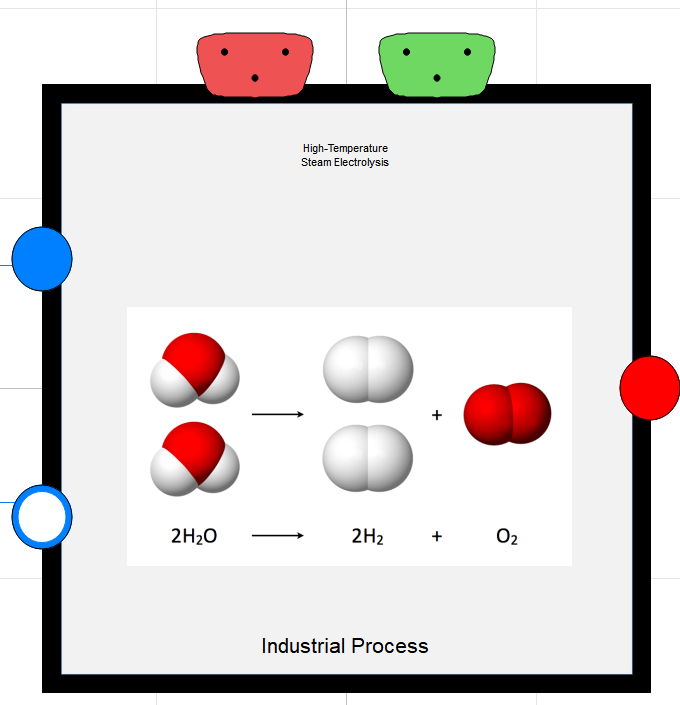
\includegraphics[scale=0.4]{pics/HTSE.png}
\caption{Top Level Depiction of the High Temperature Steam Electrolysis Unit in the NHES package}
\label{Top View HTSE}
\end{figure}



\subsubsection{Desalination}
The NHES repository includes a desalination industrial process based on reverse osmosis (RO), Figure \ref{Top View Reverse Osmosis}, designed for brackish water desalination. RO desalination utilizes a semi-permeable membrane, which allows water to pass through but not salts, thus separating the fresh water from the saline feed water. A typical Brackish Water RO (BWRO) plant consists of four main components: feed water pretreatment, High-Pressure (HP) pumping, membrane separation, and permeate (fresh water) post-treatment. The concentrate water rejected by the first membrane module plays a role as the feed water for the second membrane module by the successive order, and so on. These pressure vessels are arranged in rows in each membrane stage, with two-stage membrane separation being typical in BWRO. Each stage has a recovery of 50–60 percent, achieving overall system recovery of 70–85 percent \cite{JongDesalination}. 

The Reverse Osmosis Subsystem unit provides the user the ability to modify the number of parallel reverse osmosis units being utilized within the plant alongside to specify how much power is being input into the RO system. Each one of these parallel systems is assumed to go through a two-step the desalination process. In addition, the unit provides the user the ability to alter the salinity of the brine coming into the plant alongside a specified pressure differential across the plant. If further alterations and control are desired from a user perspective reports detailing the full specifications of the plant designs are available in \cite{2018ThermalStorage}, \cite{JongDesalination}. Additionally, base components for the entire desalination plant can be found in the “Desalination” package within the NHES repository. 
 

\begin{figure}[hbtp]
\centering
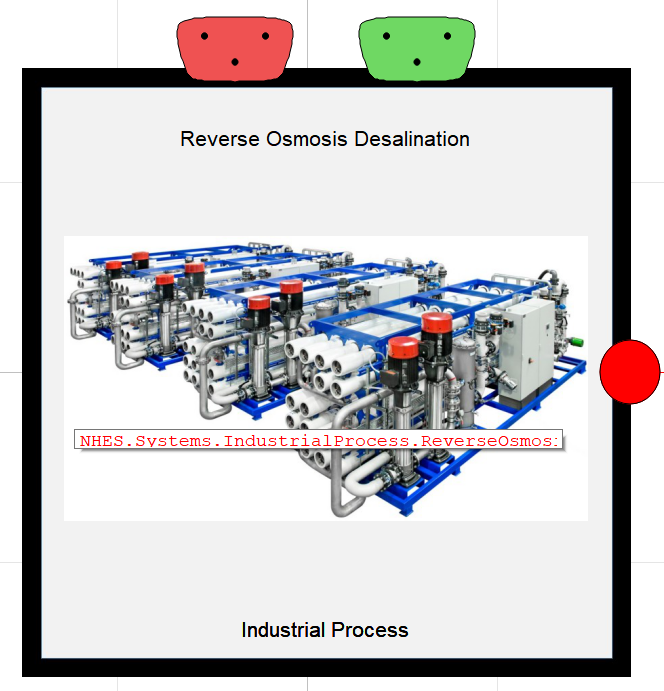
\includegraphics[scale=0.3]{pics/Desalination Plant.png}
\caption{Top Level Depiction of the Brackish Water Desalination Process in the NHES package}
\label{Top View Reverse Osmosis}
\end{figure}



% content


%\subsection{Cloning the Hybrid Repository}
\label{sec:clone raven}

The first step in installing the package is to clone the HYBRID repository. To do this, use
\begin{lstlisting}[language=bash]
git clone https://github.com/idaholab/HYBRID.git
\end{lstlisting}
This will download the repository into a folder called 'hybrid'. To go inside the folder, use
\begin{lstlisting}[language=bash]
cd hybrid
\end{lstlisting}


\subsubsection{Install RAVEN and its plugins as a sub-module}

The next step is to download and install RAVEN and the submodule (e.g. TEAL, HERON) plugins as a sub-module of the HYBRID repository. 

A submodule allows you to keep another Git repository in a subdirectory of your repository. The other repository has its own history, which does not interfere with the history of the current repository. This can be used to have external dependencies such as third party libraries for example.

In order to get RAVEN do the following in the hybrid folder

\begin{lstlisting}[language=bash]
git checkout devel
\end{lstlisting}

Update the Branch

\begin{lstlisting}[language=bash]
git pull
\end{lstlisting}

to add RAVEN as a submodule
\begin{lstlisting}[language=bash]
git submodule update --init --recursive
\end{lstlisting}

\textbf{Install and Compile RAVEN. }
Once you have downloaded RAVEN as a sub-module, you have to install it. go to the \href{https://github.com/idaholab/raven/wiki/intallationMain}{RAVEN Wiki} for information about how to install it. Run all the tests outlined in the RAVEN wiki. 

\subsubsection{Inform the Framework Paths}

In order to set up the hybrid repository, you must inform the framework about the location of the Dymola python interface. For doing so, navigate to the hybrid directory:

to add RAVEN as a submodule
\begin{lstlisting}[language=bash]
cd <path to your hybrid repository>/hybrid
\end{lstlisting}
Run the following command:
\begin{lstlisting}[language=bash]
./scripts/write_hybridrc.py -p DYMOLA_PATH
\end{lstlisting}

Where DYMOLAPATH is the path to the python interface egg folder in the DYMOLA installation locally. For example:
 
\begin{lstlisting}[language=bash]
./scripts/write_hybridrc.py -p 
	"/c/Program\ Files/Dymola\ 2020x/Modelica/Library/
	python_interface/dymola.egg"
\end{lstlisting}

